\section{Experiment}
%\begin{figure}[t]
%	\centering
%	%\fbox{\rule{0pt}{2in} \rule{0.9\linewidth}{0pt}}
%	\includegraphics[width=0.8\linewidth]{experiment.png}
%	
%	\caption{Assessing the Similarity Between Network Activation and Brain Activation.}
%	\label{fig:fig3}
%\end{figure}
%\label{sec:experiment}

\subsection{Datasets} \label{sec:Dataset}

\hspace{1pc}We conduct training and testing on Carla~\cite{Dosovitskiy:2017},
and assess the proposed BID model using existing standard datasets\cite{codevilla2019exploring}. 
Each dataset specifies its own training scenes and weather conditions for data collection, 
and tests the BID's performance in scenes never seen before. 
In behavior cloning dataset\cite{codevilla2019exploring}, they focuses on transfer ability from Town01, a small scene with numerous T junctions and a variety of buildings, to Town02, a variant of Town01 with a mixture of residential and commercial buildings.
The offical test suit presents a challenging transfer problem across 6 scenes with various scenarios, including stop signs, lane changes, US-style junctions and roundabouts.
Based on the behavior cloning dataset~\cite{codevilla2019exploring}, we test the transfer ability between different weather conditions, though only two training weather types are evaluated to save computational resources. 
The behavior cloning benchmark includes three actor amount levels for each scene from less to more. 
A crowded configuration in behavior cloning is utilized, which uses a suitable number of actors to prevent typical jam with a large number of actors. 
In the offical test suit, we adjust actor number to meet the requirement of configuration. 


% CILv2
As with the newest state-of-art model, we use the driving expert driver referred to reinforcement learning imitation~\cite{Zhang:2021} using online dataset with simulator.
This end-to-end method with reinforced feature exhibits very real action compared to a well-designed model in traffic scene. 
It is important to notice that the hoiminine driving demonstration will be used as training data in real world tests.
The standard configuration in~\cite{Zhang:2021} is used, which means that it is similar to the student driver in RL-Coach\cite{Zhang:2021} and MBI~\cite{Hu:2022}, the driving agent is the model found in simulator.
The frame from all the 3 horizontally concatenated vehicle-based RGB image sensors is 900 wide and 300 high, with a field of view of $180^{\circ}$.
The cameras are arranged without overlap, collectively covering a total filed of field.


Using the experienced agent, vehicle-based cameras and hero vehicle, driving data is collected in progressively more crowed scenarios.
Firstly, data is collected in Carla's Town01, a small scene that allows contains one lane merely, meaning we can't change lanes.
% 中午、傍晚、大雨的中午、潮湿的中午
Specifically, 1620K frames approximately at 10 fps from vehicle-based RGB sensor is utilized on 4 different learning weather types.
%: ClearNoon, ClearSunset, HardRainNoon, and WetNoon. 
% 测试:Town02 细雨的傍晚、潮湿的傍晚
For generalization testing, we use Carla's Town02, evaluating the agent under SoftRainSunset and WetSunset weather conditions. 
Next, the benchmark is collected on several simulator scene to capture crowed driving scenes, such as T junctions, highway entrances, exits, and crossing the intersections. 
To maintain consistency with setup in MBI~\cite{Hu:2022}, Town05 is reserved for testing, and totaling approximately 2,100K image per sensor is gathered at 10 fps in Town01 to Town06. 
%In Town01 and Town02, both training and testing weather conditions remain the same.



\subsection{Implementation}

\hspace{1pc}The AdamW optimizer with a step size of $2 \times 10^{-4}$ at each iteration and weight decay of $0.02$ is utilized to training the BID model. 
We reduce the learning rate by half at 25, 45, and 70 epochs.
The batch size is 100, 
and model training is performed for 100 epochs on a single NVIDIA RTX A6000 GPU.


% Cornet详细信息
In ventral stream, after the input is processed by V2$_\text{COR}$ once, the resulting output is inputted back to V2$_\text{COR}$.
This process forms a recurrent connection.
We run V2$_\text{COR}$ and IT$_\text{COR}$ two times, and execute V4$_\text{COR}$ four times repeatedly, respectively.
This configuration yielded a best model performance based on our evaluation scores.
Similar to ResNet-50, a convolutional operation is accompanied by layer normalization and a rectified linear unit.
Layer normalization is unique to each time step.
The existing description of the ventral pathway does not include the connection that span across different regions, and retinal and lateral geniculate nucleus processing are not explicitly modeled.


% 各种环境下的场景说明
% Roach_carla0913_fps10_dense_normalcamera_NoCrash_3cam/RouteScenario_0000/rgb_central001215.png
\begin{figure}[t]
	\centering
	\includegraphics[width=1.0\linewidth]{fig/dataset_examples.pdf}
	\caption{Top: When the ego-vehicle is driving on the road, even though the triffic light is green, the vehicle in front has stopped, but the ego-vehicle still brakes.
		Bottom: When the vehicle is moving and encounters a traffic jam in front, it will automaitcally brake and stop.
		The brake command in the figure is displayed in \textcolor{red}{red}.}
	\label{fig:command_ambiguous}
\end{figure}

\begin{figure}[ht!]
	\centering
	\includegraphics[width=\linewidth]{fig/structure_analysis.pdf}
	\caption{BID architecture analysis. 
		We analyse four main factors including the initial step size in ventral pathway, the number of recurrent step in dorsal pathway, the position feature dimension in VPC and the vector embedding dimension in DPC. 
		Each row presents how \emph{SR} and \emph{TL} score change based on BID when the hyperparameter changes. }
	\label{fig:structure_analysis}
\end{figure}

% 驾驶评估的3个不同数据集(不包含实验结果)
\subsection{Driving Evaluation}
\label{sec:Metrics}
\hspace{1pc}The BID agent's capabilities are constrained by the proficiency of the expert it is emulating. 
The success of the agent hinges on the expertise and skill level of its human counterpart.
If the expert performs poorly, the agent that mimics it will also show suboptimal results. 
The BID model is designed to closely follow the visual information processing system of the human brain, both structurally and functionally. 
When optimized, the model's output closely matches the expert's performance, as evaluated by similarity metrics.


We conduct experiments on small single-lane town following the nocrash dataset~\cite{Zhang:2021,Hu:2022}, and on multiple towns (Sec.~\ref{sec:small_town_results}) based on the offline Carla leaderboard dataset~\cite{Zhang:2021,Hu:2022}. 


% 三种不同场景的性能
\begin{table*}
	\caption{Results in Town02.
		The expert refers to reinforcement learning~\cite{Zhang:2021}, while RL-Coach refers to Coach imitation learning. 
		Carla is used to evaluate all methods.
		3 experiment with various random seeds are used to calculate the mean values and standard deviations.
		Better performance is indicated by higher values for metrics marked with $\uparrow$, while lower are perferred for those marked with $\downarrow$.}
	\centering
	\resizebox{0.95\linewidth}{!}{
		\begin{tabular}{@{}lccc|ccc|ccc@{}}
			\hline
			& \multicolumn{3}{c}{None} & \multicolumn{3}{c}{Normal} & \multicolumn{3}{c}{Crowded}  \\
			
			& SR(\%,$\uparrow$) & SSR(\%,$\uparrow$) &  TL($\downarrow$)  & SR(\%,$\uparrow$) & SSR(\%,$\uparrow$) &  TL($\downarrow$) & SR(\%,$\uparrow$) & SSR(\%,$\uparrow$) & CV($\downarrow$) \\
			\hline
			
			RL-Coach\cite{Zhang:2021}  & $100\pm0.0$ & $85\pm1.2$ & $66\pm5.0$ & $97\pm2.3$ & $86\pm7.2$ & $66\pm54$ & $81\pm5.0$& $68\pm7.2$ & $63\pm52.7$\\
			MVA\cite{xiao2023scaling} & $100\pm0.0$ & $100\pm0.0$ & $0\pm0.0$  & $99\pm2.3$ & $97\pm3.1$ & $7\pm7.9$ & $83\pm7.6$ & $77\pm7.6$ & $45\pm21.5$ \\
			Our BID & $100\pm0.0$ & $100\pm0.0$ & $0\pm0.0$  & $99\pm2.3$ & $97\pm3.1$ & $7\pm7.9$ & $83\pm7.6$ & $77\pm7.6$ & $45\pm21.5$ \\
			\hline
			Expert & $100\pm0.0$ & $100\pm0.0$ & $0\pm0.0$ & $100\pm0.0$ & $97\pm0.0$ & $13\pm4.6$ & $84\pm2.0$ & $82\pm2.0$ & $37\pm14.1$ \\
			\hline 
		\end{tabular}
	}
	\label{tab:T2_NC_results}
\end{table*}


\begin{table*}
	\caption{Town05 outcomes based on offline measurements.
		Carla is used to evaluate all methods.
		3 experiment with various random seeds are used to calculate the mean values and standard deviations.
		Better performance is indicated by higher values for metrics marked with $\uparrow$, while lower are perferred for those marked with $\downarrow$.}
	\centering
	\resizebox{0.87\linewidth}{!}{
		\begin{tabular}{@{}lccccccccccccccccccccc@{}}
			\hline
			%   & SR(\%) 
			%   & S.SR(\%) 
			& $\uparrow$ APA(\%) & $\uparrow$ ADG
			& $\downarrow$ CV & $\downarrow$ CL & $\downarrow$ TL & $\downarrow$ OL & $\downarrow$ RD 
			\\
			\hline
			RL-Coach\cite{Zhang:2021}  & $92\pm3.1$ & $51\pm7.9$ 
			& $7.5\pm1.3$ & $4.3\pm1.6$ & $26.0\pm8.9$ & $5.4\pm2.7$ & $3.0\pm3.2$ & \\
			MBI~\cite{Hu:2022}
			& $98\pm2.2$ & $73\pm2.9$ 
			& $6.0\pm3.7$ & $0.0\pm0.0$ & $3.6\pm3.8$ & $3.5\pm1.5$ & $0.0\pm0.0$ \\   
			MVA\cite{xiao2023scaling} 
			& $98\pm1.7$ & $68\pm2.7$ 
			& $6.0\pm0.5$ & $3.8\pm0.7$ & $5.8\pm5.1$ & $6.1\pm2.2$ & $9.4\pm3.6$ \\
			Our BID 
			& $98\pm1.7$ & $68\pm2.7$ 
			& $6.0\pm0.5$ & $3.8\pm0.7$ & $5.8\pm5.1$ & $6.1\pm2.2$ & $9.4\pm3.6$ \\
			\hline
			Expert 
			& $99\pm0.8$ & $89\pm1.7$ 
			& $3.2\pm1.1$ & $0.0\pm0.0$ & $1.3\pm0.4$ & $0.0\pm0.0$ & $0.0\pm0.0$ \\
			\hline
		\end{tabular}
	}
	\label{tab:T5_results}
\end{table*}

\subsubsection{Official Measurement}\label{lb_metrics}
\hspace{1pc}We utilize the officiial measurement in several simulation scenes in order to match the evaluation with Carla leaderboard\cite{Hu:2022}.
% Avg.DS 平均驾驶分数、平均路线完成
The average path accomplishment (\emph{APA}) and the average drive grade (\emph{ADG}) are the most important measurement index. 
While \emph{APA} measures the average distance that the agent can run toward the goal,
\emph{ADG} penalizes driving performance according to the criteria outlines for the Carla measurement.
% Avg.RC:自车辆能够行驶至目标的平均距离。


% 高层导航命令
\subsubsection{Goal Instruction} 
\hspace{1pc}During training, we employ basic goal instructions like ``turn left" or ``go straight" when reaching a crossroad, just like in LBC\cite{Codevilla:2019}.
After passing a crossroad in more complex scenes, the ego-vehicle maybe legal when entering one of the several available routes. 
Because these information is avaiable through the global navigation system, if the vehicle agent departs from the pre-designed trajectory by entering a different lane, a corrected command is given, such as ``turn right" or ``turn left" as quickly as feasible. 
The corrected method is applied during evaluating merely.
An example of this process is shown in Fig.~\ref{fig:command_ambiguous}.


\subsubsection{Nocrash Benchmark Evaluation}\label{nocrash_metrics}

\hspace{1pc}Based on the quantity of variational actors ({\ie}, human, cars) in Carla scene, the benchmark comprises 3 mission with varying degrees of challenge: crowded, normal and none.
Town02 specifies that there are zero human and zeros cars (none); fifty human and fifteen cars (normal); and one hundred fifty human and seventy cars (crowded).
%
% 默认的配置会导致拥堵死锁
The initial actors quantity in nocrash benchmark frequently causes crowded and congestion at intersections in the crowded scenario~\cite{Zhang:2021}.
To address this, we adopt the \emph{crowded} scenarios described in RL-Coach~\cite{Zhang:2021}, reducing human population from one hundred and fifty to seventy. 
%A task consist of two weather conditions never seen it before and twenty-five goal-oriented scenarios.
%If a crash happens, the simulated case ends is considered a failure.
%The driving rate is penalized for unexpected violations in accordance with the guidelines outlined in these benchmark.


% 度量标准的说明
The success rate (\emph{SR}), which represents the proportion of runs that are normally finished, is the primary evaluation index for comparing agents.
% 严格的成功率
We also offer the rigorous \emph{SR} (\emph{SSR}) for a more detailed measurement, which calculates the proportion of normal runs under a 0 violation policy for any rules, like running at a no passing traffic sign or deviating from planned route.
% T.L:在红灯时不停的次数
Additionally, we include other violative measurement.
The quantity of vehicle that fails to stop at a red traffic sign is represented by \emph{TL}.
% 和其他车辆碰撞的次数
The quantity of crashes with other cars is denoted by \emph{CV}.
% R.Dev:当高层命令没有很好地执行,路线偏差的次数
The quantity of path inconformity where the high level navigation is not properly run is denoted by \emph{RD}.
% O.L:考虑了自主车辆驶出车道的情况(例如,在对面车道或人行道上)
\emph{OL} is the quantity of the agent deviate from its lane ({\eg}, to the sidewalk or to the opposite lane).
% C.L:与城镇布局发生碰撞的次数
The quantity of crashes with scene is symbolized by \emph{CL}.
%Per kilometer driving, we normalize all the number of violations.




\subsection{Experiment Result}
\label{sec:Results}
% 基于模型的模仿学习
\hspace{1pc}We contrast BID with three state-of-the-art, vision-based AD models: the Coach IL method (here RL-Coach) \cite{Zhang:2021}, MBI~\cite{Hu:2022} and MVA\cite{xiao2023scaling}. 
It is important to note that while BID employ sample produced by the RL-Coach method, optimizing a BID doesn't need image annotated by humans. 
In this instance, the RL-Coach model acts as the experienced driver during sample collection.
On the other hand, BID is trained using segmented Bird's Eye View (BEV) data as input, whereas BID model needs supervised signal from RL-Coach driver, who learned from real world data, while MBI is optimized.


\subsubsection{One lane Scenes} \label{sec:small_town_results}

\hspace{1pc}Using one lane scenes in Carla and  the nocrash evaluations, firstly we perform preliminary experiments (Sec.~\ref{nocrash_metrics}). 
We employ Town01 to train BID, and use Town02 to evaluate our proposed model(Sec.~\ref{sec:Dataset}). 
MBI offers one that has been optimized on multiple simulator scenes, while no model is available that is specifically trained on Town01 alone. 
On the other hand, RL-Coach is a model optimized with various simulator scenes. 
We employ RL-Coach's model optimized on Town01 merely to ensure a reasonable evaluation. 
The \emph{SR} and \emph{SSR} with the different actor quantities (none, normal, crowded) are shown in Table~\ref{tab:T2_NC_results}. 
To provide a targeted assessment, we report \emph{IRL} (infractions with red light) in the none and normal scenarios, and \emph{CWV} (collisions with vehicles) merely for the crowded case in Table~\ref{fig:score_eu_lb_tt_tn}. 
It is important to emphasize that scenarios with fewer or no dynamic obstacles are more effective for evaluating the agent's response to red traffic signs, whereas crashes are appropriately assessed in towns with higher traffic density.


Generally speaking, BID performs the best performances across various missions. 
When it comes to avoiding traffic sign violations in the none case, BID performs noticeably better than RL-Coach, which raises the \emph{SSR}.
This conclusion holds true in a normal scenario as well. 
BID comes close to matching the expert's performance in the crowded scenario, outperforming RL-Coach in terms of \emph{SSR} and resulting in fewer crashes with cars again. 
According to the ground truth, scenario that failed in crowded runs are primarily cause of actors blocking up, which cause a timeout during path finish. 
Despite this, the expert's performance can still be considered a valid upper bound.


\subsubsection{Multi-scene Transferability}\label{sec:multi_towns_result}
\hspace{1pc}We evaluate the result of BID in increasingly intricate runs that Carla numerous scenes provide in the part. 
We use Carla official benchmark measurements (Sec.~\ref{lb_metrics}) and align the train and test settings with those used in MBI~\cite{Hu:2022}, as outlined in Sec.~\ref{sec:Dataset}. 
Table~\ref{tab:T5_results} displays the outcomes for every method that was optimized using multi-scene dataset. 
Out of the 3 methods, RL-Coach performs the least, incurring more violations and resulting in a noticeably smaller \emph{ADG}. 
APA of 98\% attained by BID is comparable to MBI. 
However, MBI has the highest \emph{ADG} score (73\%), while BID achieves 68\%. 
We attribute this difference to the fact that MBI rarely drives outside the pre-designed lane, as it is provided with the route map as input. 
In contrast, BID does not use an explicit route map and instead relies solely on high level  goal instructions.

% 不同迭代时的消融实验
% CILv2_multiview\network\models\architectures\CIL_multiview\evaluator.py
\begin{figure*}[t]
	\centering
	\includegraphics[width=0.99\textwidth]{fig/driving_scores.pdf}
	\vspace{-1ex}
	\caption{\textbf{Driving performance and training progress of BID.} 
		All BID agents are evaluated in LBCRoutes after 30 peoch.
		Top figure: The ground truth and model prediction for steering angles are shown in green and blue, respectively.
		Bottom figure: The errors in training progress are displayed every 5 epochs, including the mean absolute error (MAE) for steering and acceleration.
		While other metrics are tested with single random number, we describe the outcome as the averaged value over 5 test random number.
		For evaluation, the offical benchmark is employed.}
	\vspace{-1.5ex}
	\label{fig:score_eu_lb_tt_tn}
\end{figure*}


% 在密集场景中的消融实验
% table:sucess_rate_nc_dense
\begin{table}
	\caption{\textbf{Camera-based imitation learning agent's \emph{SR} on crowded environments.}
		The mean value and deviation are computed based on 5 random seeds. 
		% 数据聚合方法:DAGGER:试图在学习策略诱导的状态分布下收集专家演示
		% Our models are from DAGGER iteration 5. 
		NCC: nocrash-crowded. ts: train scene. tw: train scene and weather have never seen before. ns: new scene. nw: new scene and weather have never seen before.
		In EDA, ``(E)" denotes an assembly of iteration sets, while ``+" indicates the additive jitter on the benchmark.}
	\setlength{\tabcolsep}{6.67pt}
	\centering
	\begin{tabular}{lccccc}
		\hline
		\emph{SR} \% $\uparrow$
		& NCC-tw  & NCC-ts   & NCC-nw  & NCC-ns  \\ 
		\hline
		% \cmidrule(lr){1-1}\cmidrule(lr){2-5}
		SMN \cite{zhao2021sam} & 
		$48 \pm 4$ & $53 \pm 2$  & $30 \pm 3$ & $30 \pm 2$  \\
		LC \cite{chen2020learning} & 
		$64 \pm 2$ & $69 \pm 4$  & $40 \pm 5$ & $52 \pm 2$  \\
		LSD \cite{ohn2020learning} & 
		N/A & N/A & $31 \pm 4$ & $31 \pm 3$  \\
		EDA \cite{prakash2020exploring} & 
		$57 \pm 2$ & $65 \pm 4$  & $36 \pm 1$ & $37 \pm 2$  \\
		EDA\textsuperscript{+} \cite{prakash2020exploring}  & 
		$61 \pm 2$ & $61 \pm 2$  & $26 \pm 2$ & $35 \pm 1$  \\
		Baseline, $\mathcal{L}$ & 
		$30 \pm 2$ & $\mathbf{87} \pm 2$  & $29 \pm 5$ & $35 \pm 9$  \\
		Improved, $\mathcal{L}_\text{D} $ & 
		$31 \pm 1$ & $\mathbf{87} \pm 1$  & $29 \pm 4$ & $33 \pm 10$  \\
		Proposed, $\mathcal{L}_\text{D}+\mathcal{L}_\text{N}$ & 
		$\mathbf{83} \pm 3$ & $86 \pm 3$  & $\mathbf{79} \pm 1$ & $\mathbf{79} \pm 4$  \\
		\hline
	\end{tabular}
	\vspace{-1ex}
	\label{table:sucess_rate_nc_dense}
	\vspace{-2ex}
\end{table}

\begin{table*}
	\caption{\textbf{Analyzing BID's output effect and infractions in scene never seen it before with a lot of people.} 
		IP: infraction penalty. CWO: collision with others. CWP: collision with pedestrian. 
		CWV: collision with vehile.
		IRL: infraction with red light.
		ABD: agent blocked.
		5 test random number seeds are employed to display the mean value and deviation.}
	\setlength{\tabcolsep}{7.4pt}
	\centering
	\begin{tabular}{lccccccccc} 
		\hline
		& \begin{tabular}{@{}c@{}} DS ($\uparrow$) \end{tabular} 
		& \begin{tabular}{@{}c@{}} SR ($\uparrow$)  \end{tabular} 
		& \begin{tabular}{@{}c@{}} IP ($\uparrow$) \end{tabular} 
		& \begin{tabular}{@{}c@{}} PA ($\uparrow$)  \end{tabular} 
		& \begin{tabular}{@{}c@{}} ABD ($\downarrow$) \end{tabular} 
		& \begin{tabular}{@{}c@{}} IRL ($\downarrow$) \end{tabular} 
		& \begin{tabular}{@{}c@{}} CWO ($\downarrow$) \end{tabular}  
		& \begin{tabular}{@{}c@{}} CWP ($\downarrow$) \end{tabular}  
		& \begin{tabular}{@{}c@{}} CWV  ($\downarrow$) \end{tabular}  \\
		\hline
		% \cmidrule(lr){1-1}\cmidrule(lr){2-5}\cmidrule(lr){6-10}
%		iter 5
%		& \%, $\uparrow$
%		& \%, $\uparrow$
%		& \%, $\uparrow$
%		& \%, $\uparrow$
%		& \#/Km, $\downarrow$
%		& \#/Km, $\downarrow$
%		& \#/Km, $\downarrow$
%		& \#/Km, $\downarrow$
%		& \#/Km, $\downarrow$
%		\\
%		\hline
		%\cmidrule(lr){1-1}\cmidrule(lr){2-5}\cmidrule(lr){6-10}
		$\mathcal{L}_\mathrm{b}$
		& $42 \pm 3$ & $32 \pm 5$  & $76 \pm 4$ & $61 \pm 5$  
		& $19.4\pm 14.4$ & $3.33 \pm 0.58$  & $0.53 \pm 0.55$  & $\mathbf{0}\pm0$ & $0.63 \pm 0.50$    \\
		$\mathcal{L}_D$
		& $65\pm3$ & $58\pm6$  & $76\pm1$ & $85\pm2$  
		& $2.83\pm1.46$ & $1.5\pm0.2$  & $2.06\pm1.28$  & $\mathbf{0}\pm0$ & $1.37\pm1.10$    \\
		$\mathcal{L}_N$
		& $90\pm2$ & $85\pm1$ & $75\pm2$  & $78\pm0$  
		& $3.36\pm0.21$ & $0.69\pm0.06$ & $0.51\pm0.25$  & $\mathbf{0}\pm0$  & $0.52\pm0.17$    \\
		$\mathcal{L}_D+\mathcal{L}_N$
		& $89 \pm 3$ & $88 \pm 5$  & $90 \pm 3$ & $\mathbf{97} \pm 0$  
		& $0.83 \pm 0.03$ & $0.62 \pm 0.22$ & $\mathbf{0.07} \pm 0.04$  &  $0.01 \pm 0.01$ & $0.22 \pm 0.07$    \\
		%\hline
		%\cmidrule(lr){1-1}\cmidrule(lr){2-5}\cmidrule(lr){6-10}
		$\mathcal{L}_{BID}$
		& $\mathbf{96} \pm 2$ & $\mathbf{96} \pm 3$ & $96 \pm 0$ & $97 \pm 2$ 
		&  $\mathbf{0} \pm 0$ & $\mathbf{0.14} \pm 0.18$  & $0.12 \pm 0.08$  & $\mathbf{0} \pm 0$  & $\mathbf{0.03} \pm 0.06$  \\
		Expert
		& $91 \pm 1$ & $78 \pm 2$ & $\mathbf{97} \pm 1$ & $81 \pm 2$ 
		& $0.19 \pm 0.07$ & $1.92 \pm 0.22$  & $0.19 \pm 0.07$ & $\mathbf{0} \pm 0$ & $0.17 \pm 0.09$   \\
		\hline
	\end{tabular}
	\vspace{-1ex}
	\vspace{-2.5ex}
	\label{table:infraction}
\end{table*}


% 可视化注意力
\subsubsection{BID's Activation Visualization}
\label{sec:Visualization}
\hspace{1pc}We want to know which parts of the image BID focuses on during decision-making. 
To achieve this, we use Grad-CAM~\cite{Selvaraju:2017}, where gradients from driving behavior embedding to last convolution in ResNet-50. 
The process generates the heatmap that identifies the areas of frame that are most crucial for driving behavior generation. 
Nevertheless, Grad-CAM was initially created in frame recognition task, where outcomes are often positive, whereas BID handles regressive mission, so the outcome can take both positive and negative values.
We can't just concentrate on the representation map's positive gradients to modify Grad-CAM for these situation.
Instead, the calculation is split into 2 scenarios according to the outcome value's symbol. 
We employ negative gradient to compute a feature map weights when the steering angle or acceleration is negative, and positive gradients are used when the output is positive.


% _results\_results\CILv2\CILv2_3cam_single_lane\Eval\Valid_gradCAM_Roach_LBCRoutes_3cam_valid\30\-1\85.jpg
Fig.~\ref{fig:attention_ped_greed} illustrates the attention image in a crossroad. 
3 regions of the frame are most noticed: a lane shoulder on the frame right, the human crossing the street in the frame center, and the driving area on the frame left. 
This suggests that BID demonstrates a thorough comprehension of the scenario and a discernible connection between its observations and actions. 
Specifically, BID chooses to slow down because of the crossing human, despite the green traffic sign and the goal instruction is to turn left. 
This indicates that BID appropriately prioritizes the presence of pedestrians over the traffic signal and navigation command.


% 验证集的1350帧,激活图的第45张
\begin{figure}[ht!]
	\centering
	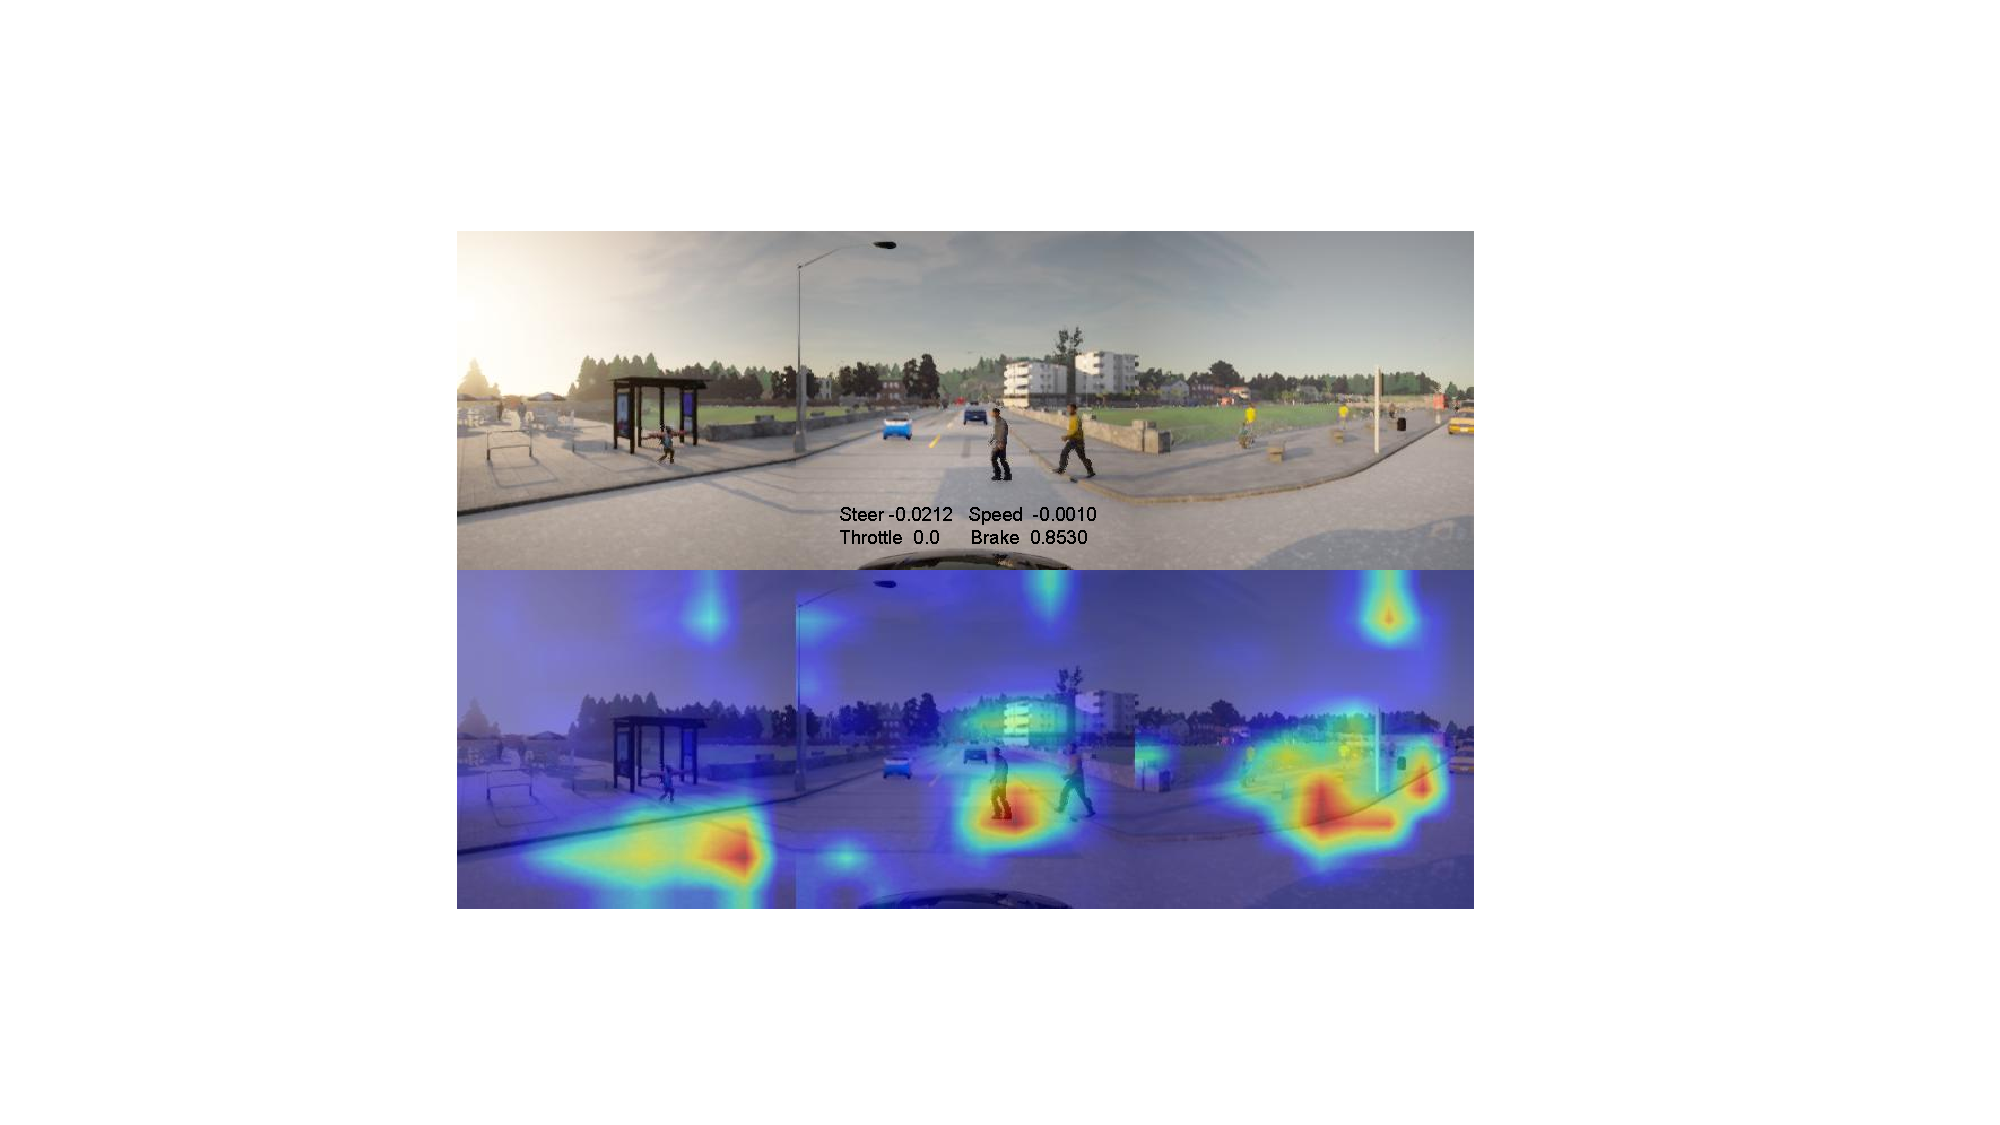
\includegraphics[width=\linewidth]{fig/attention_ped_greed.pdf}
	\caption{Activation maps of BID at an intersection in Town02 show three highly activated image areas from driving viewpoints: 
		the lane shoulder in the right, the crossing pedestrians in the center, and the driving area in the left. 
		The causality between observation and action is demonstrated by a strong braking response (0.8530) due to the presence of pedestrians, despite the ``go-straight" command. 
		This highlights BID's ability to prioritize pedestrian safety over other factors in BID's decision-making process. }
	\label{fig:attention_ped_greed}
\end{figure}



% 消融实验:速度(包括背侧通路)、导航
\subsubsection{Ablation}

\hspace{1pc}An imitation learning ego-vehicle's ability to perform is inherently constrained by the quality of experienced driver it imitates. 
Comparing imitation learning ego-vehicle trained on an experienced driver is pointless if that driver performs poorly.
This issue becomes apparent in a scenario never seen it before with crowded actors, where the performance of autopilot typically is poor. 
We optimize the BID (Fig.~\ref{fig:score_eu_lb_tt_tn}) and conduct ablation studies with architecture analysis (Fig.~\ref{fig:structure_analysis} and the crowded actors configuration (Table~\ref{table:infraction}) to establish a high precision effect and ensure a effective evaluation, allowing the proposed agent to attain a \emph{DS} of 96\%. 
As shown in Table~\ref{table:sucess_rate_nc_dense}, the optimal configuration from the ablative experiments is also assessed on benchmark in crowded actors for a more meaningful comparison with latest models.


% 说明消融的各个指标?
% L_N 导航信号
% L_D 背侧流信号
Fig.~\ref{fig:score_eu_lb_tt_tn} shows the behavior grades of experienced and imitation learning drivers for an epoch on offical benchmark with crowded actors.
The basic $\mathcal{L}$ represents the proposed implementation of the baseline BID trained by expert. 
According to the leaderboard instructions, this additional navigation vector helps separating scenes where the map's complexity may make it difficult to understand the labels of each frame.
Given the improvements in our best-performing BID, it is expected that $\mathcal{L}_D$ and $\mathcal{L}_D + \mathcal{L}_N$ gain better \emph{SR} than results described in Table~\ref{table:sucess_rate_nc_dense}.
The significant performance gap between the baseline and $\mathcal{L}_D + \mathcal{L}_N$, especially when transferring to the scene never seen it before, highlights the basic approach limitations.


% 一步步添加后的效果
$\mathcal{L}_D$ outperforms $\mathcal{L}_b$ overall by incorporating the dorsal stream and speed embedding into the baseline $\mathcal{L}_b$.
Additionally, learning from the action distribution allows $\mathcal{L}_D$ to generalize superior than $\mathcal{L}_b$ on the benchmark dataset, but not on the offical leaderboard.
When $E_S$ is given merely, the feature required to generate accurate driving action does representation mapping to enhance performance.
Since the expected path is given throught nagivation command in this instance, $E_N$ includes goal instructions.
The use of $E_N$ improves accuray for the benchmark because it encodes goal instruction, including the feature pointing to the following expected path.
To evaluate this idea, we utilize a integrated model structure in which the goal instruction described as one hot encoding is added to the evaluation feature $E_N$.
In the benchmark scene transferability evaluation, $\mathcal{L}_\text{BID}$ achieves the highest behavior degree in imitation learning ego-vehicles.



%
Adding supervised representation alongside feature matching accelerates the convergence of the process, as demonstrated by $\mathcal{L}_D + \mathcal{L}_N$.
However, when feature matching is omitted, supervised representation doesn't lead to better result with $\mathcal{L}_D$.
These suggests the possibility of value estimation and representation mapping working in tandem.
Predicting the value should be made easier by imitating the representation of RL-coach, which intuitively contains the feature needed for value prediction. 
In turn, these estimation can be enhanced by regularizing representation mapping, improving overall performance.


\subsubsection{Infraction and Result Analysis}


\hspace{1pc}Table~\ref{table:infraction} presents a particular result and infraction analyse on the benchmark dataset with crowded actors in the scene never seen it before. 
Interestingly, the remarkably better \emph{ABD} degree in the basic $\mathcal{L}_b)$ is primarily caused by results from heavy rains. 
The issue is significantly reduced by imitating expert leading to a 23\% absolute improvement in the \emph{DS} for $\mathcal{L}_D$.
While maintaining the same IL strategy, this gain illustrates the advantages of using a more knowledgeable driver. 
Better improvements are achieved with the addition of soft targets and latent feature supervision in $\mathcal{L}_D+\mathcal{L}_N$, resulting in another 30\% absolute increase in performance. 
By handling red lights more effectively, this BID agent achieves a driving score of 89\%, reaching expert-level performance with just camera image as input.





 